\documentclass{beamer}

\usetheme{Warsaw}
\usecolortheme{rose}
\useoutertheme[]{sidebar}
\setbeamercovered{transparent}
\usepackage[slovak]{babel}
\usepackage[T1]{fontenc}
\usepackage[utf8]{inputenc}
\usepackage{url}
\usepackage{listings}

\lstset{language=C++,basicstyle=\fontsize{8}{9.6}\selectfont,showstringspaces=false,columns=fullflexible,identifierstyle=\ttfamily,keywordstyle=\bfseries,showstringspaces=false,columns=fullflexible}

\newcommand{\footcite}[1]{\footnote{\tiny #1}}
\newcommand{\umlet}{.5}
\newcommand{\emp}[1]{\textit{\alert{#1}}}
\newcommand{\kw}[1]{\mbox{\textbf{#1}}}
\newcommand{\id}[1]{\texttt{#1}}
\newcommand{\stl}{\guillemotleft}
\newcommand{\str}{\guillemotright}

\newcommand{\lsti}{\lstinline[basicstyle=\fontsize{10.5}{12.1}\selectfont]}

\newenvironment{program}{\begin{beamercolorbox}[rounded=true,shadow=true]{block body}\vspace{-4mm}}{\vspace{-2mm}\end{beamercolorbox}}

\setbeamercolor{fvystup}{fg=white,bg=black}
\newenvironment{vystup}{\begin{beamercolorbox}[rounded=true,shadow=true]{fvystup}}{\end{beamercolorbox}}

\newenvironment{poznamka}{\begin{beamercolorbox}[rounded=true,shadow=false]{block body}}{\end{beamercolorbox}}

\setbeamertemplate{footline}[page number]
{
%\insertpagenumber
%\begin{beamercolorbox}{section in head/foot}
%\vskip2pt\insertnavigation{\paperwidth}\vskip2pt
%\end{beamercolorbox}%
}



\author{Anton Dmitriev}
\institute{Slovenská Technická Univerzita v Bratislave}
\title{Ako Funguje Vyhľadávanie Online Máp}
\subtitle{\vspace{3mm} Metódy Inžinierskej Práce 2023/2024}
\date{\today}


\begin{document}

\begin{frame}
\titlepage
\end{frame}


\begin{frame}[fragile=singleslide]\frametitle{O čom to je?}
Tento článok je informačným zdrojom, ktorý vysvetľuje aspekty online mapovania a predstavuje pohľad na zmeny, ktorými táto oblasť prešla.
\\Motiváciou na napísanie tohto článku bol môj hlboký záujem o technologické inovácie v oblasti digitálneho kartografovania a želanie sprístupniť tieto údaje ľuďom.
\end{frame}


\begin{frame}[fragile=singleslide]\frametitle{Prehľad}
\tableofcontents
\end{frame}


\section{História vývoja online máp}

\begin{frame}[fragile=singleslide]\frametitle{Krátke pozadie kartografie}
V roku 1569 vynašiel kartograf Gerardus Mercator refolučnú projekciu, ktorá sa dodnes používa vďaka schopnosti zobraziť zemeguľu na štvorcovej ploche.
\begin{figure}[h]
	\centering
	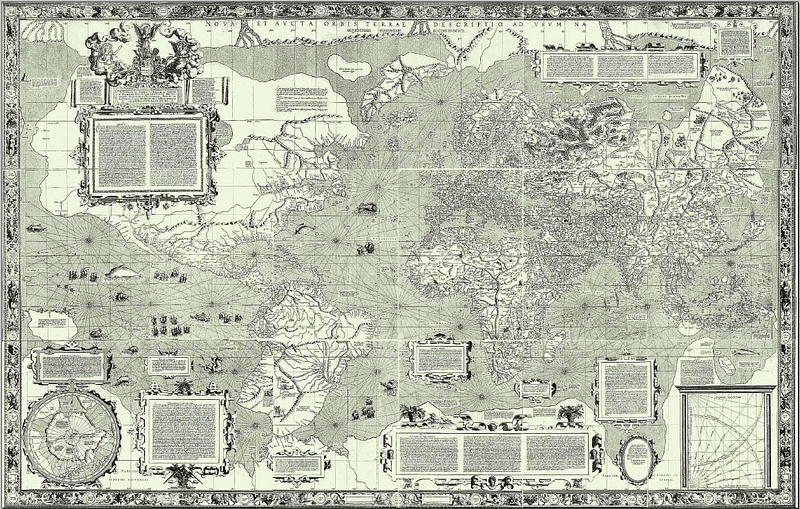
\includegraphics[scale=0.25]{image1.png}
	\caption{Mercatorova mapa sveta z roku 1569}
	\label{fig:mercator}
\end{figure}
\end{frame}

\begin{frame}[fragile=singleslide]\frametitle{Mapy Google: Zmena hry}
Spoločnosť Google vstúpila na trh online máp v roku 2005 uvedením služby Google Maps, ktorej úspech spočíval v množstve inovatívnych funkcií.
\begin{figure}[h]
	\centering
	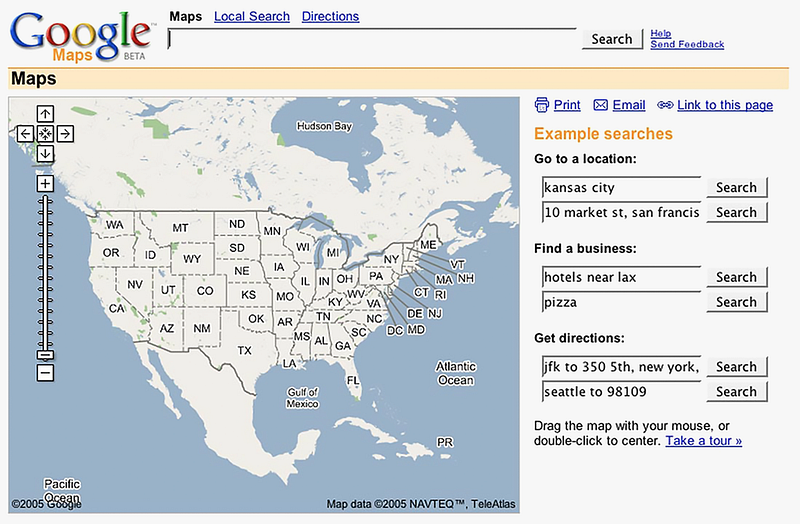
\includegraphics[scale=0.25]{image2.png}
	\caption{Google Maps na začiatku}
	\label{fig:googlemaps}
\end{figure}
\end{frame}


\section{Interná štruktúra}

\begin{frame}[fragile=singleslide]\frametitle{Najkratšia cesta z bodu A do bodu B}
Online mapy používajú grafovú dátovú štruktúru na rýchly výpočet najkratšej cesty. Na tento účel sa používa Dijkstrov algoritmus.
\begin{program}
\begin{lstlisting}[language=C, caption=Reprezentácia pseudokódu]
function  dijkstraAlgorithm(graph, source):
	for each node n in graph:
		distance[n] := infinity
		previous[n] := undefined
	distance[source] := 0
	q := the set of all nodes in graph
	while q is not empty:
		z := node in q with smallest distance[ ]
		remove z from q
		for each unvisited neighbor n of z:
			dist := distance[u] + dist_between(z, n)
			if dist < distance[n]
				distance[n] := dist
				previous[n] := z
return distance[ ] previous[ ]
	
\end{lstlisting}
\end{program}
\end{frame}

\begin{frame}[fragile=singleslide]\frametitle{Čo je to geokódovanie?}
\begin{columns}
	\begin{column}{0.5\textwidth}
	Geokódovanie je proces prevodu adries (napr. "Prokopa Veľkého 41, Bratislava, Slovensko") na geografické súradnice (zemepisnú šírku a dĺžku), ktoré možno použiť na umiestnenie značiek na mapu alebo na určenie polohy mapy.
	\end{column}
		
	\begin{column}{0.5\textwidth}
	\begin{figure}[h]
		\centering
		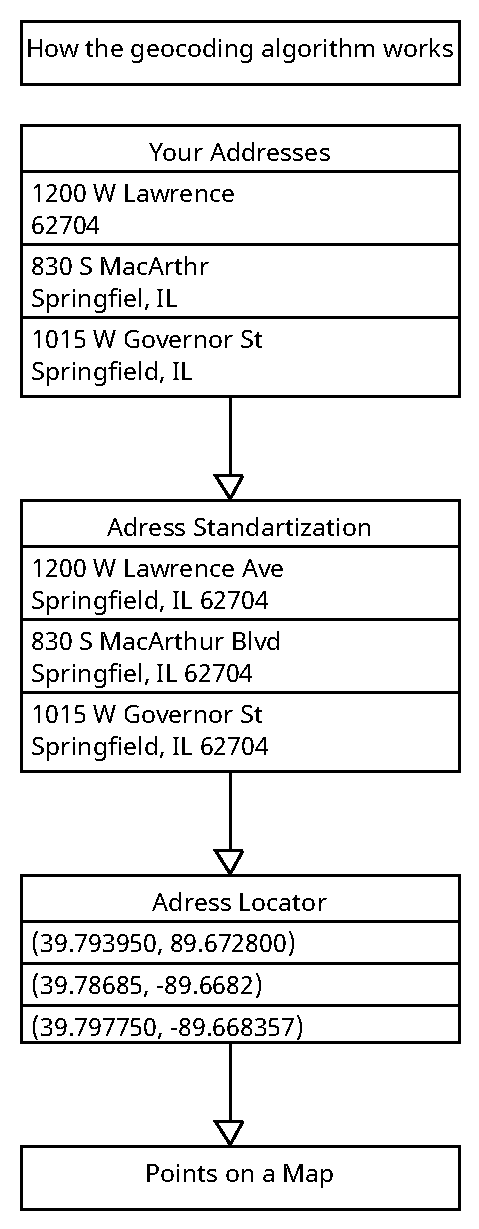
\includegraphics[scale=0.27]{diagram1.pdf}
		\caption{Proces geokódovania}
		\label{fig:geocoding}
	\end{figure}
	\end{column}
\end{columns}
\end{frame}

\begin{frame}[fragile=singleslide]\frametitle{Zisťovanie polohy: Nemôžete sa pred ňou skryť}
Globálny polohový systém (GPS) - je satelitný systém vo vlastníctve vlády USA, ktorý poskytuje používateľom služby určovania polohy, navigácie a časovania. Systém GPS funguje vďaka trilaterácii.
\begin{figure}[h]
	\centering
	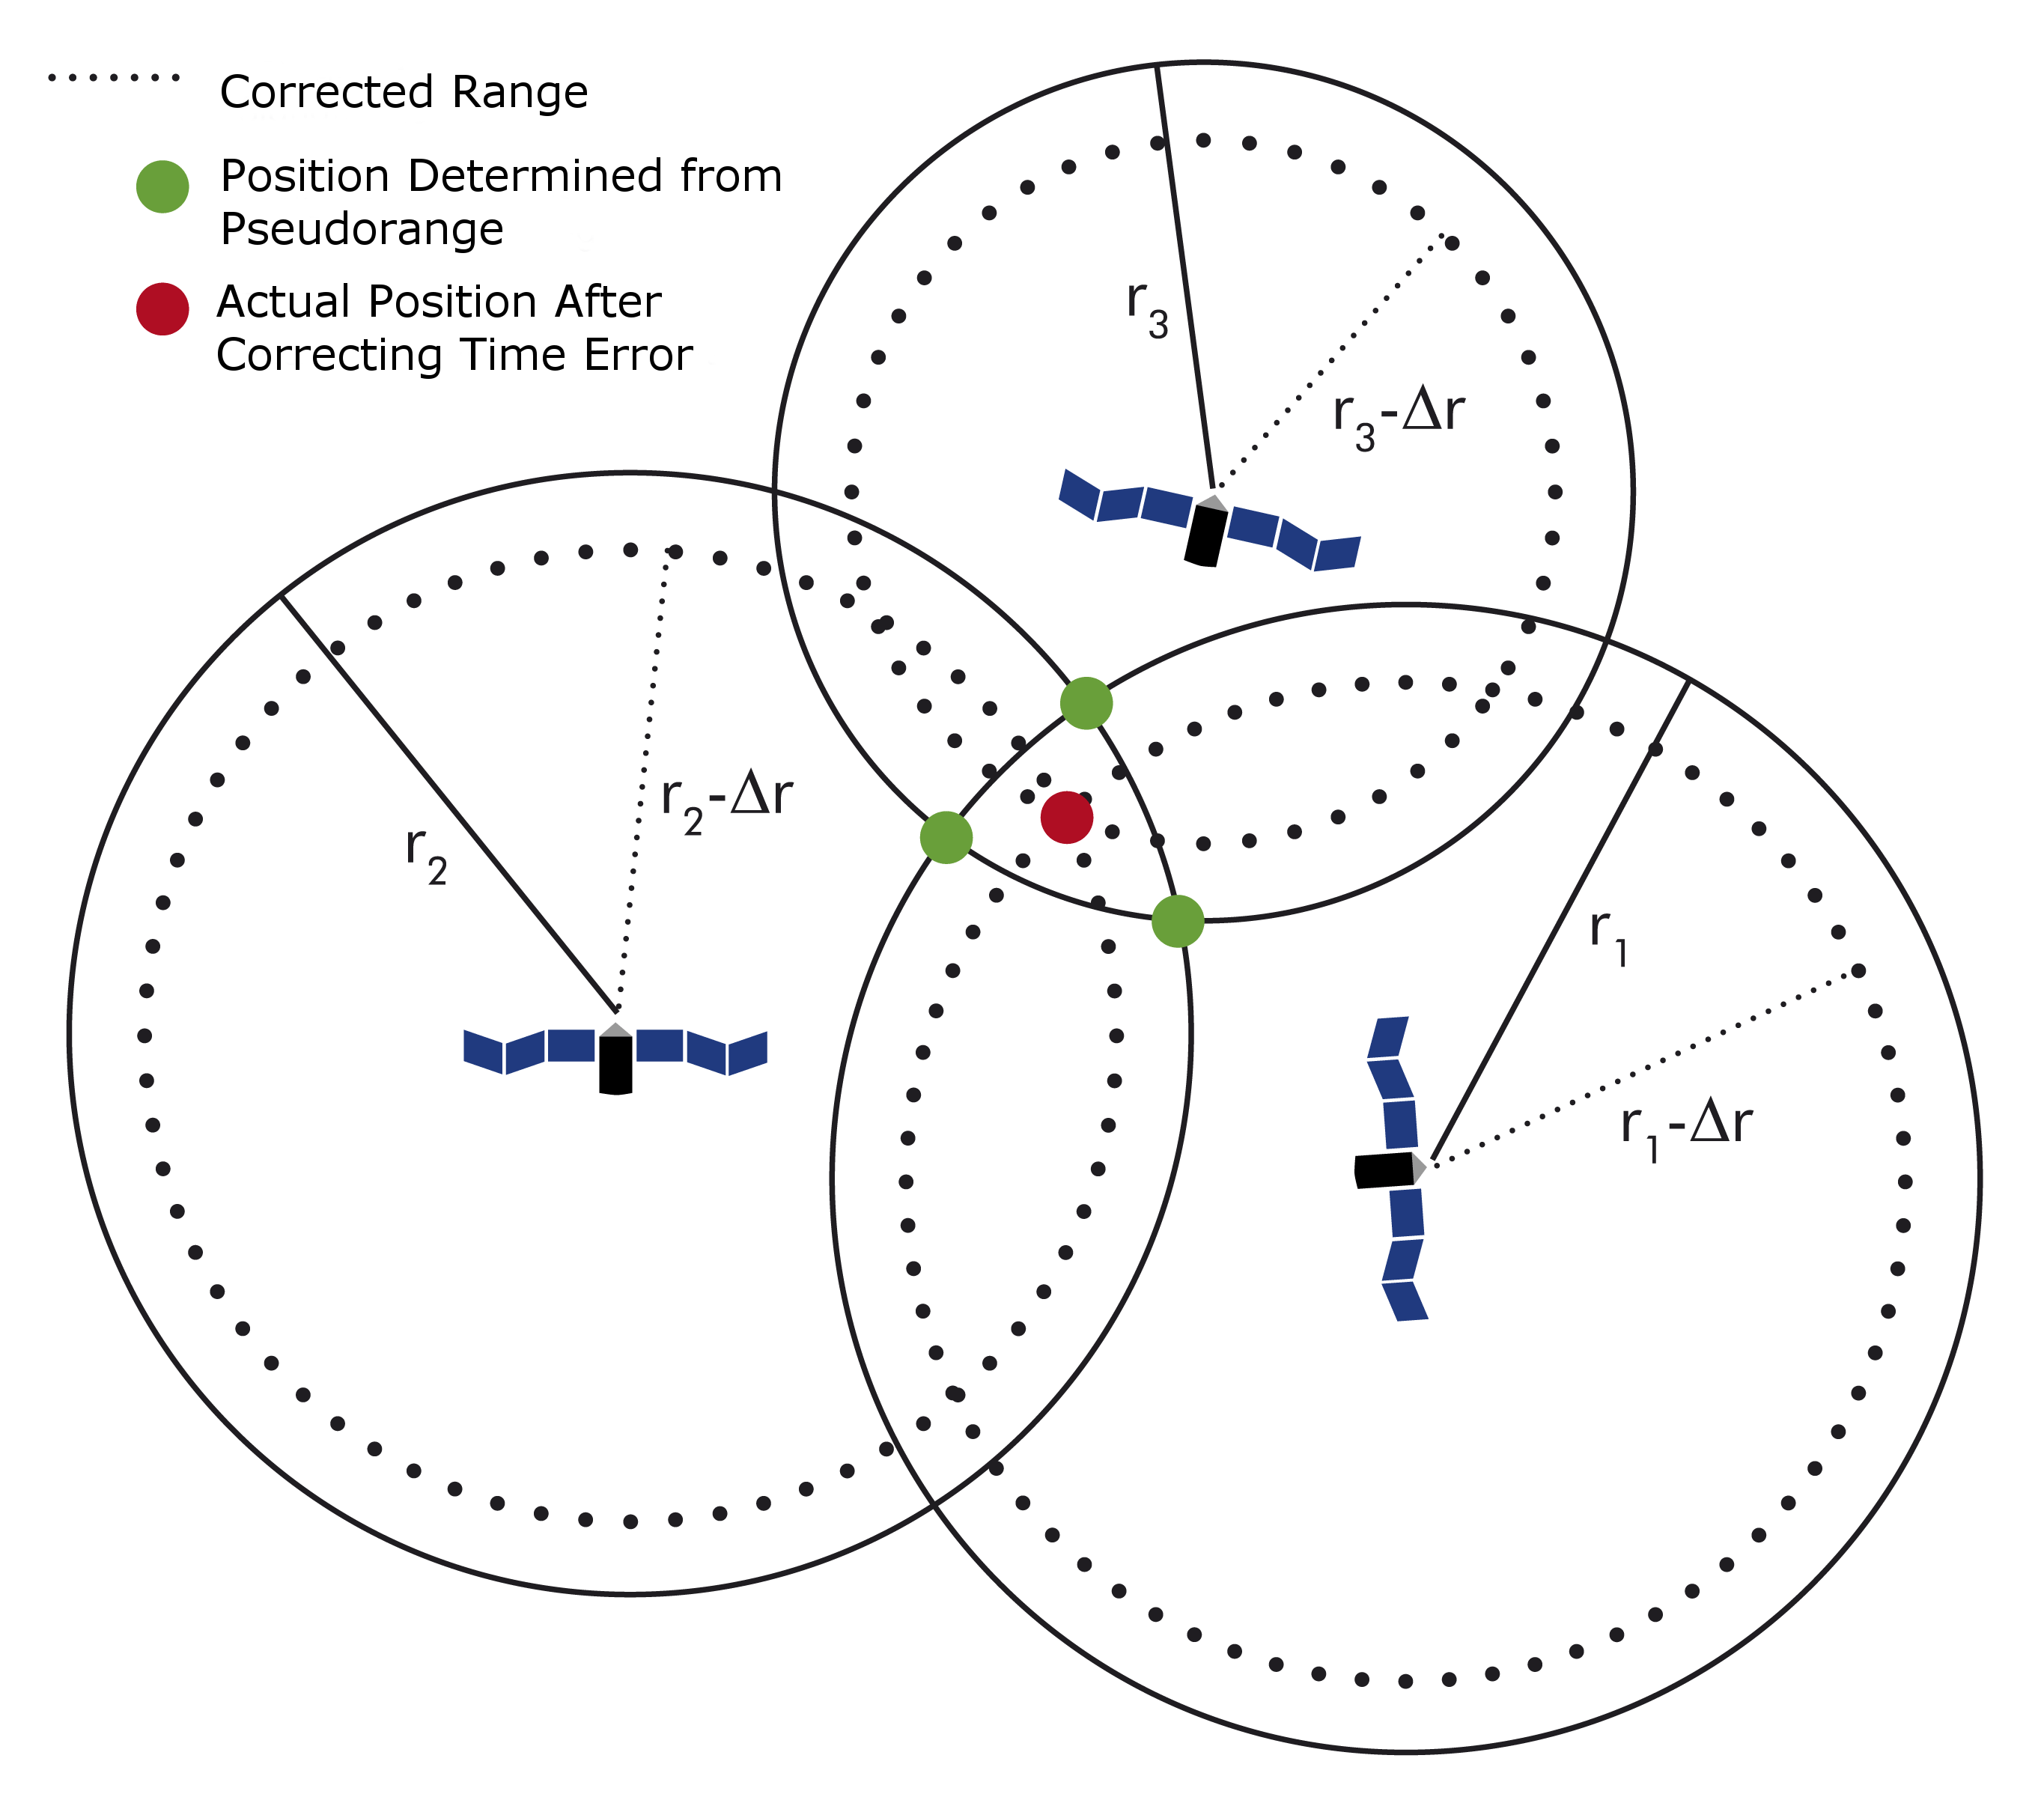
\includegraphics[scale=0.05]{diagram3.png}
	\caption{Vizuálny príklad sústavy 3 satelitov GPS}
	\label{fig:trilateration}
\end{figure}
\end{frame}

\section{Dátová štruktúra}

\begin{frame}[fragile=singleslide]\frametitle{Čo je GIS?}
Geografické informačné systémy (GIS) sú komplexné nástroje, ktoré zbierajú, ukladajú, spracúvajú, analyzujú a vizualizujú údaje súvisiace s konkrétnymi geografickými koordinátmi.
\begin{figure}[h]
	\centering
	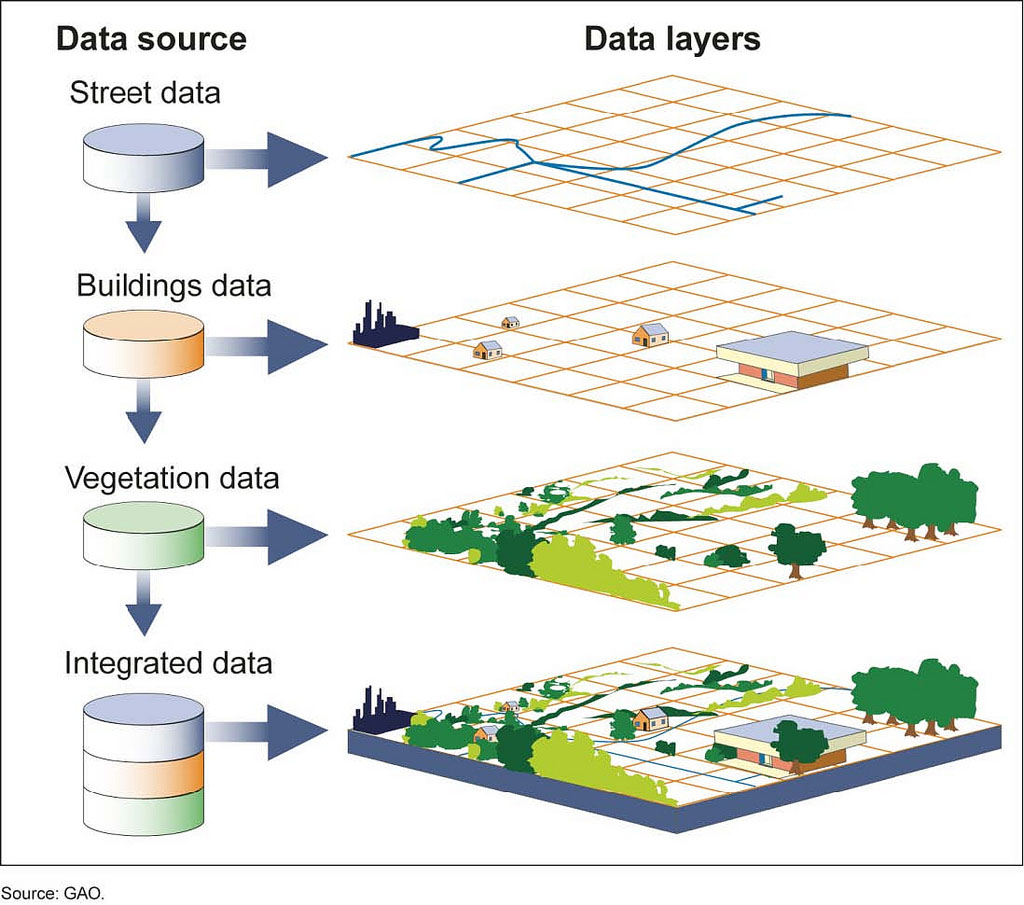
\includegraphics[scale=0.4]{image3.jpg}
	\caption{Vizualizácia rôznych úrovní GIS}
	\label{fig:gis}
\end{figure}
\end{frame}

\begin{frame}[fragile=singleslide]\frametitle{Typy údajov GIS}
\begin{columns}
	\begin{column}{0.5\textwidth}
		\begin{figure}[h]
			\centering
			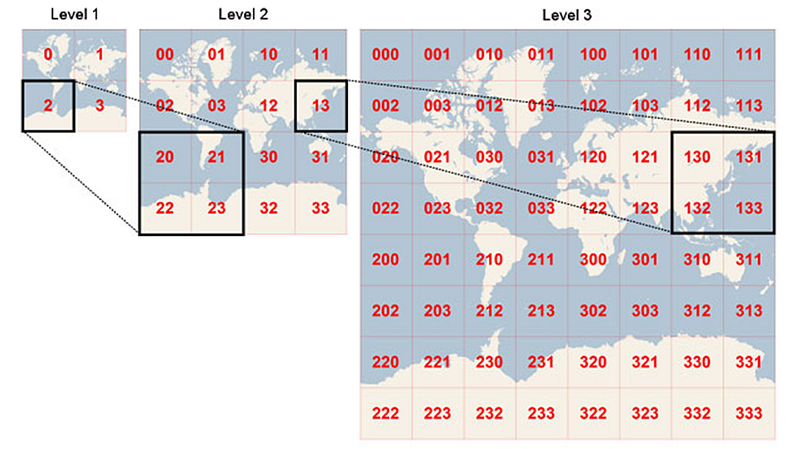
\includegraphics[scale=0.2]{diagram5.png}
			\caption{Rastrové dáta}
			\label{fig:raster}
		\end{figure}
	\end{column}
	
	\begin{column}{0.5\textwidth}
		\begin{figure}[h]
			\centering
			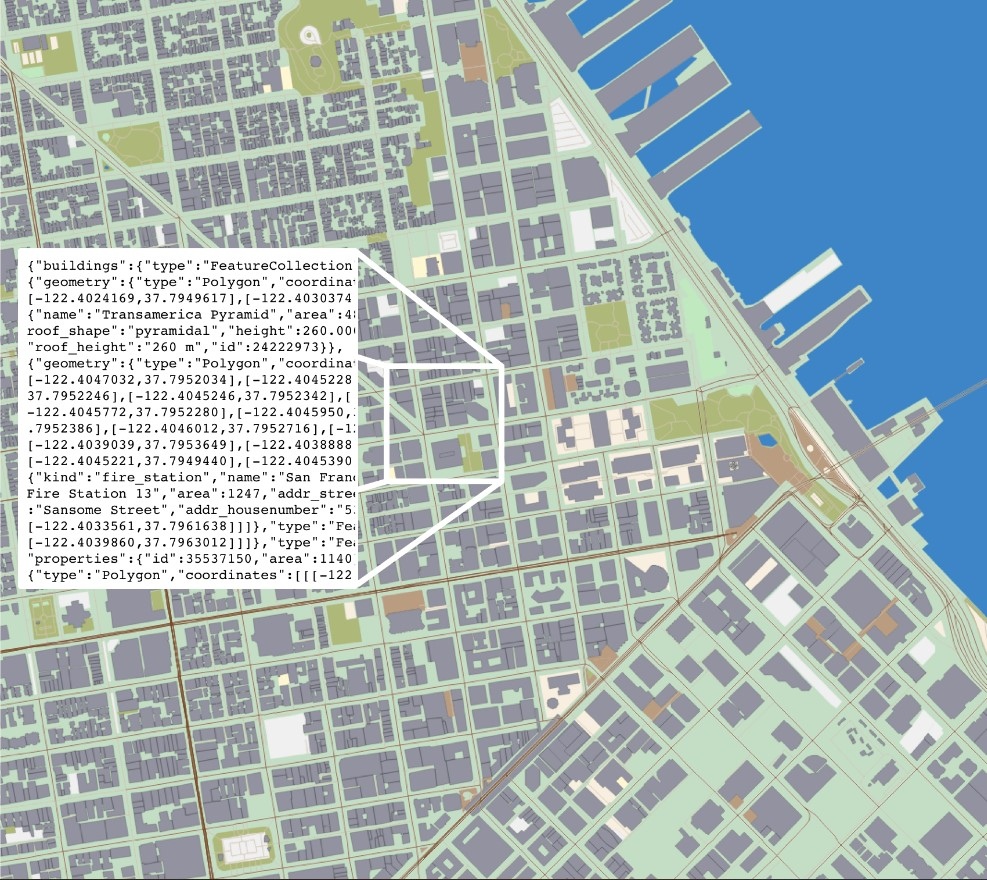
\includegraphics[scale=0.2]{diagram6a.jpg}
			\caption{Vektorové dáta}
			\label{fig:vector}
		\end{figure}
	\end{column}
\end{columns}
\end{frame}

\section{Budúcnosť online mapovania}

\begin{frame}[fragile=singleslide]\frametitle{Integrácia technológií rozšírenej reality}
Integrácia technológií rozšírenej reality do online máp môže obohatiť vizuálny zážitok používateľa poskytnutím interaktívnych 3D modelov a rozšírených údajov o lokalite v reálnom čase.
\begin{figure}[h]
	\centering
	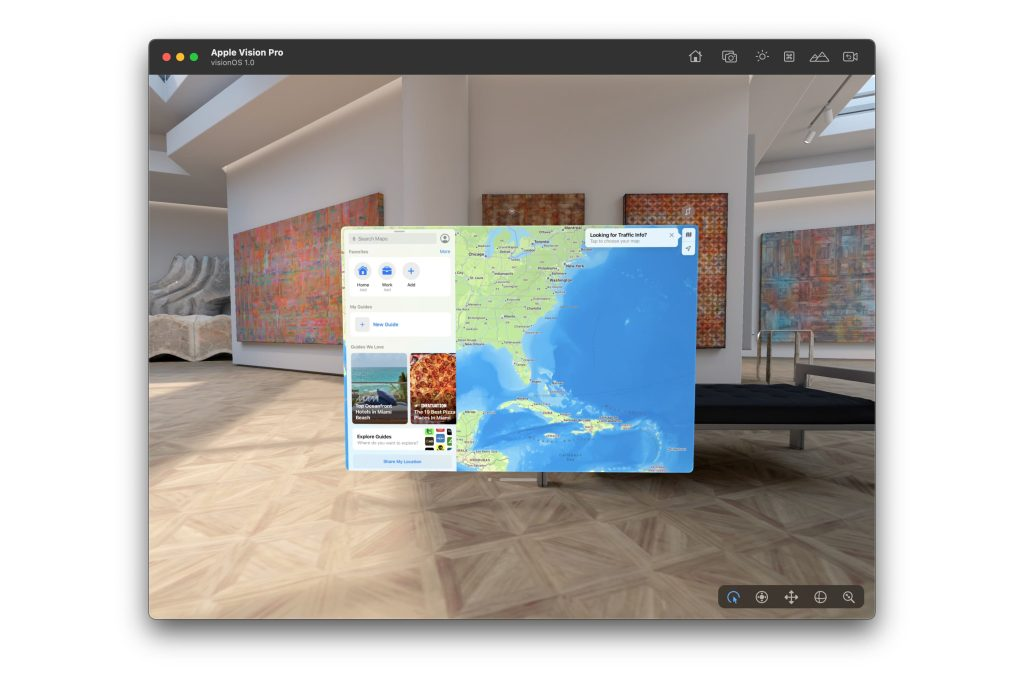
\includegraphics[scale=0.2]{diagram7.jpg}
	\caption{Online mapy v rozšírenej realite}
	\label{fig:ar}
\end{figure}
\end{frame}

\begin{frame}[fragile=singleslide]\frametitle{Integrácia do samojazdiacich vozidiel}
Samojazdiace vozidlá spoločnosti Google ukazujú, ako sa integrujú online mapy a senzory LiDAR: tieto vozidlá využívajú údaje z Google Maps na poskytovanie informácií o stave ciest a rýchlostných limitoch, zatiaľ čo senzory poskytujú informácie o aktuálnych dopravných problémoch. 
\begin{figure}[h]
	\centering
	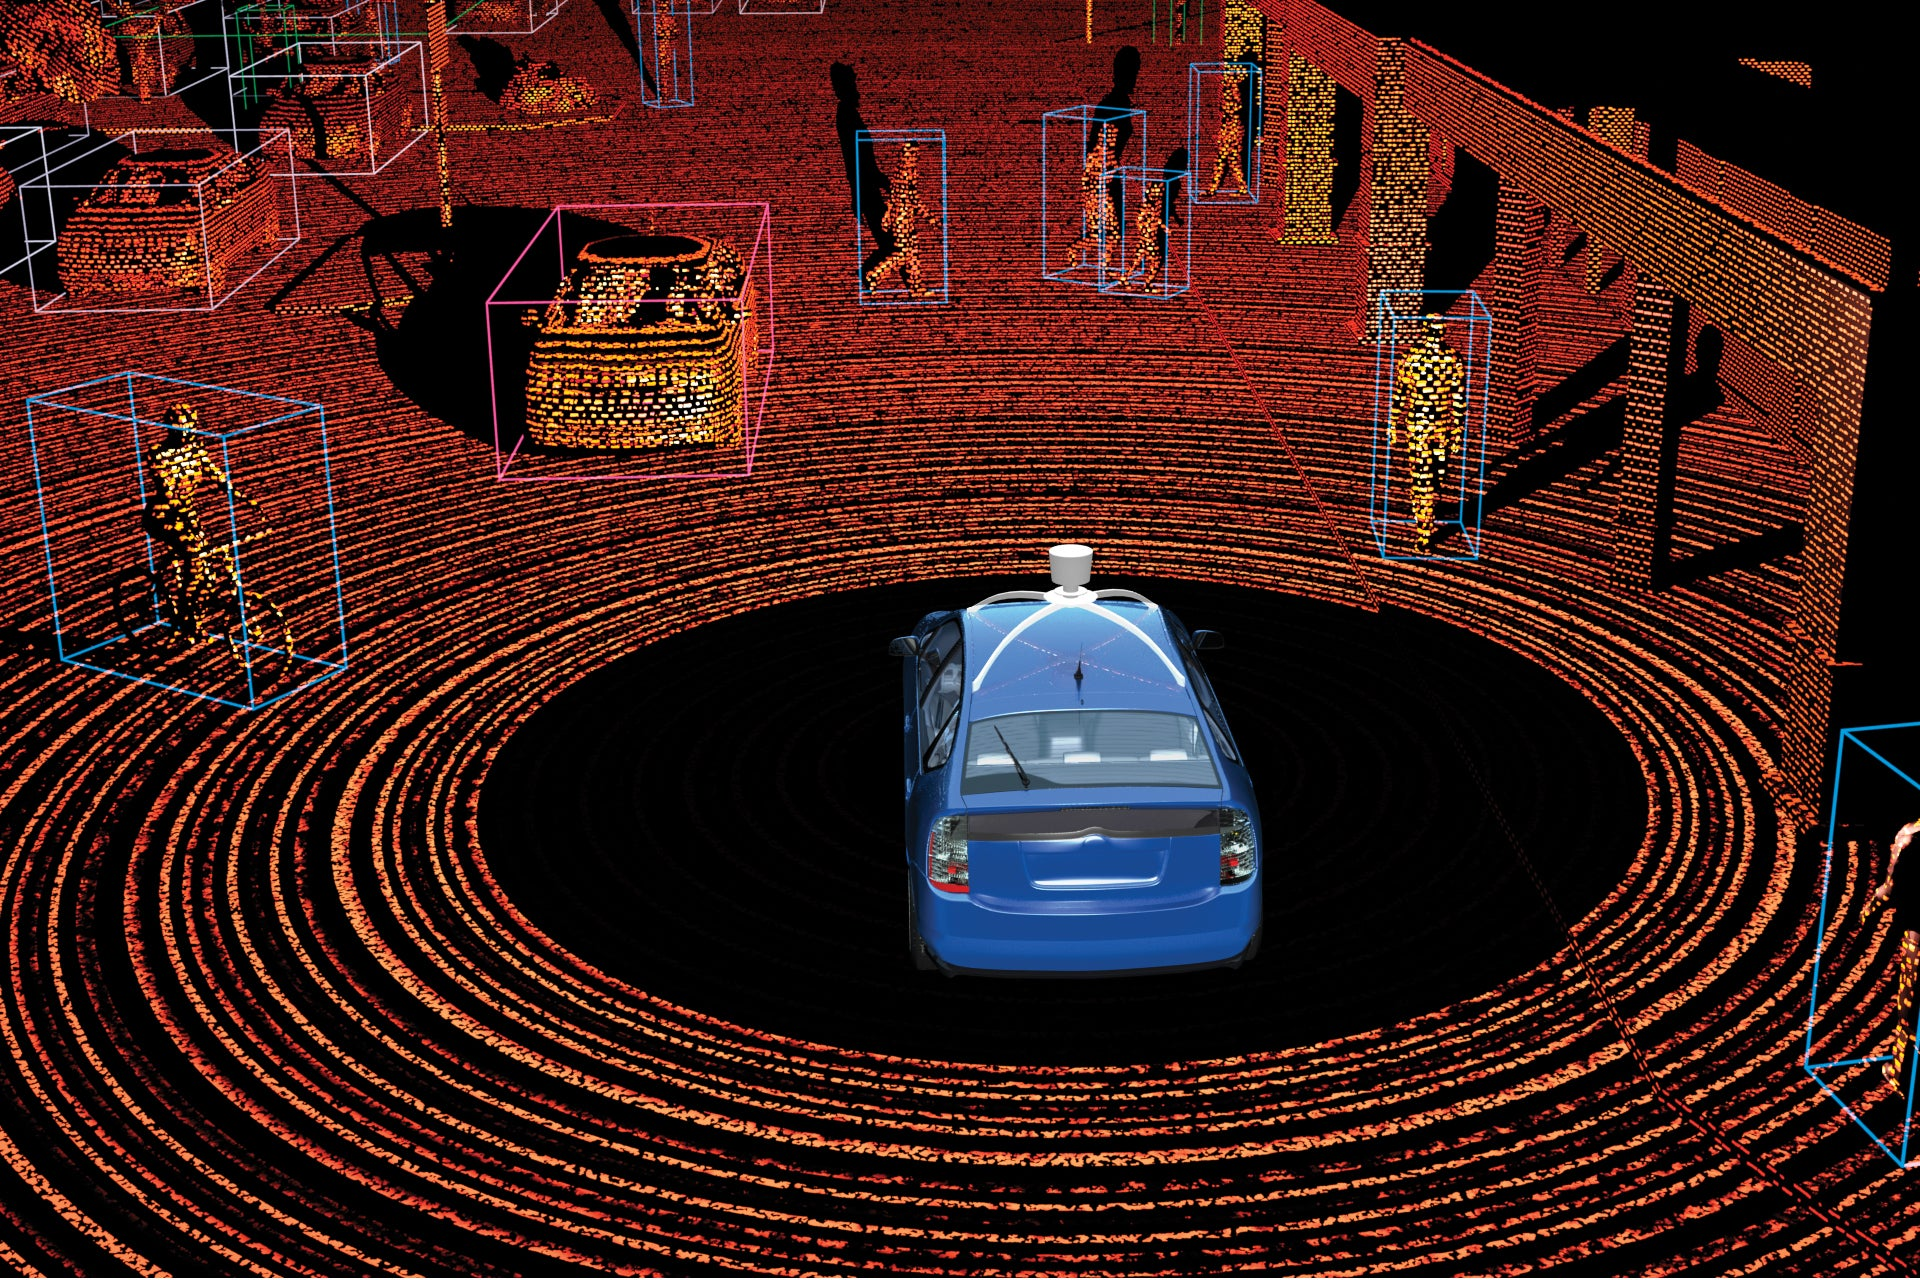
\includegraphics[scale=0.08]{image4.jpg}
	\caption{Samojazdiace auto získava reálne údaje o svojom okolí}
	\label{fig:car}
\end{figure}
\end{frame}

\begin{frame}[fragile=singleslide]\frametitle{Integrácia umelej inteligencie na vytváranie mapových údajov}
V dnešnom svete sa technológie umelej inteligencie rozvíjajú nevídaným tempom a otvárajú nové obzory v mnohých oblastiach, napríklad pri generovaní obrázkov na základe textových opisov zadaných používateľom. 
	\begin{figure}[h]
		\centering
		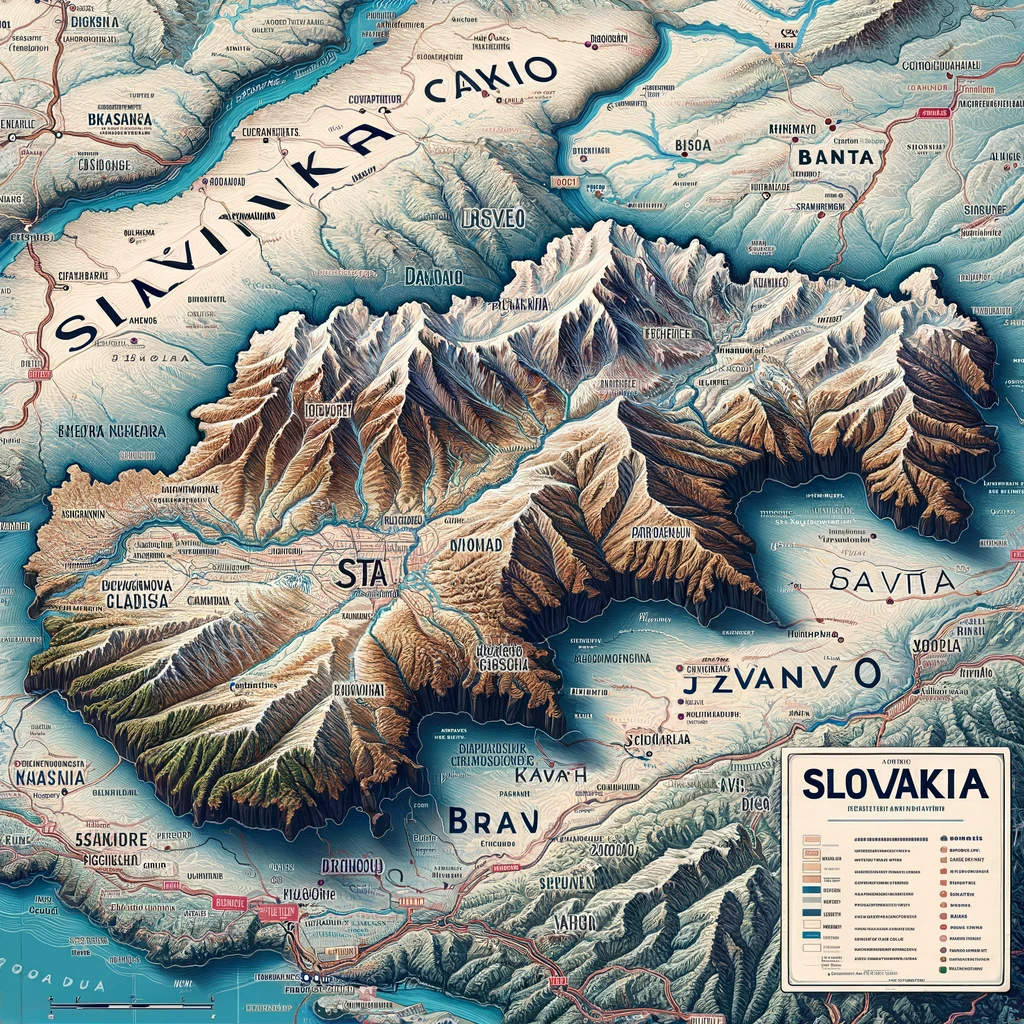
\includegraphics[scale=0.12]{image6.png}
		\caption{Mapa Slovenska nakreslená umelou inteligenciou}
		\label{fig:ai}
	\end{figure}
\end{frame}

\section*{Zhodnotenie a ďalšia práca}

\begin{frame}[fragile=singleslide]\frametitle{Zhodnotenie a ďalšia práca}
Na záver sme sa povrchne pozreli na to, ako online mapy prešli značnými zmenami, ktoré používateľom výrazne uľahčili vyhľadávanie správnych lokalít. Vo svojej budúcej práci budem ďalej rozvíjať tému článku a zameriam sa na hlbšie štúdium algoritmov online máp. 
\end{frame}


\end{document}

